\section{Theorie}
\label{sec:Theorie}
\subsection{Magnetische Momente von Elektronen und Atomen}
Der Gesamtdrehimpuls eines Elektron der Elektronenhülle setzt sich zusammen aus seinem Bahndrehimpuls $\vec{l}$ und seinem Spin $\vec{s}$.
Der Spin wird hierbei als eine Art Eigendrehimpuls betrachtet.
Für beide ergibt sich aus den Eigenwertgleichung unter Verwendung der zugeorneten Quantenzahlen $l$ und $s$:
\begin{gather}
  |\vec{l}|=\sqrt{l\left(l+1\right)}\hbar \mathrm{;}\\
  |\vec{s}|=\sqrt{s\left(s+1\right)}\hbar \mathrm{.}\\
\end{gather}
Beiden ist aufgrund der Elektronenladung ein magnetisches Moment zugeordnet.
Eine Drehimpulseinheit definiert hierbei das sogenannte Bohrsche Magneton:
\begin{equation}
  \mu_{\mathrm{B}}=-\frac{1}{2}e_0\frac{\hbar}{m_0}=\mu_{\mathrm{l}}(m=1)
\end{equation}
Mit dem Bohrschen Magneton ergeben sich die magnetischen Momente des Bahndrehimpulses $\mu_{\mathrm{l}}$ und des Spins $\mu_{\mathrm{s}}$ zu:
\begin{gather}
  |\vec{\mu_{\mathrm{l}}}|=-\mu_{\mathrm{B}}\sqrt{l\left(l+1\right)}\mathrm{;}\\
  |\vec{\mu_{\mathrm{s}}}|=-\mu_{\mathrm{B}}g_{\mathrm{S}}\sqrt{s\left(s+1\right)}\mathrm{.}
\end{gather}
Es ist hierbei $\hbar$ das Planksche Wirkungsquantum und $g_{\mathrm{S}}$ der sogenannte Landé-Faktor. Dieser berücksichtigt, dass die gemessenen magnetischen Momente des Spins
etwa doppelt so groß sind wie die theoretisch berechneten Werte des magnetischen Moments zum Spin des Elektrons nach der klassischen Physik. Der Landé-Faktor des Elektrons ist daher etwa 2. Dies wird auch als die magnetomechanische Anomalie des Elektrons bezeichnet.
Die Betrachtung von Atomen mit mehr als einem Elektron in der Elektronenhülle stellt sich als recht kompliziert heraus, da von jedem Elektron der Elektronenhülle
wechselseitig alle Drehimpulse und Spins aufeinander wirken. Es werden daher zumeist zwei häufig vorkommende Grenzfälle betrachtet.
\subsubsection{Leichte Atome (Niedrige Kernladungszahl)}
Bei Atomen mit wenigen Elektronen koppeln die einzelnen Bahndrehimpulse $\vec{l}_i$ viel stärker aneinander, als an die zugehörigen Spins der Elektronen. Es ergibt sich daher der Gesamtbahndrehimpuls der Elektronenhülle aus der Summe der einzelnen Bahndrehimpulse:
\begin{equation}
  \vec{L}=\sum_i{\vec{l}_i}\mathrm{.}
\end{equation}
Dem Gesamtbahndrehimpuls ist hierbei der Eigenwert $|\vec{L}|=\sqrt{L\left(L+1\right)} \hbar$ zugeordnet.
In der Summe müssen hierbei lediglich die Bahndrehimpulse von Elektronen auf nicht abgeschlossenen Schalen beachtet werden, da sich die Bahndrehimpulse von abgeschlossenen Schalen zu Null addieren.
Dem Gesamtbahndrehimpuls $\vec{L}$ ist das magnetische Moment $|\vec{\mu_{\mathrm{L}}}|=\mu_{\mathrm{B}}\sqrt{\mathrm{L}\left(\mathrm{L}+1\right)}$ zugeordnet.
Die Betrachtung der Spins erfolgt analog. Mit der Summe über die Spins der Elektronen auf nicht abgeschlossenen Schalen $\vec{S}=\sum_i{\vec{s}_i}$
ergibt sich der Gesamtspin der Elektronenhülle.
Mit dem zugehöriger Eigenwert $|\vec{S}|=\sqrt{S\left(S+1\right)}\hbar$
ergibt sich das magnetische Moment erneut unter Verwendung des Landé-Faktors zu:
\begin{equation}
  |\vec{\mu_{\mathrm{S}}}|=\mathrm{g_S}\mu_{\mathrm{B}}\sqrt{\mathrm{S}\left(\mathrm{S}+1\right)}
\end{equation}
Sofern die betrachteten Atome nicht zu großen Magnetfeldern unterliegen, ergibt sich der Gesamtdrehimpuls zu $\vec{J}=\vec{L}+\vec{S}$.
Mit der Quantenzahl $J$ ist der zugehörige Eigenwert $|\vec{J}|=\sqrt{J(J+1)}\hbar$ gegeben.
Diese Kopplung der Drehimpulse wird als \textbf{Russel-Saunders-Kopplung} bezeichnet.
\subsubsection{Schwere Kerne(große Kernladungszahl)}
Bei schweren Kernen tritt die sogenannte \textbf{j-j-Kopplung} auf.
Da bei schweren Kernen die Elektronenschalen, welche nicht voll besetzt sind, relativ weit weg vom Atomkern sind, sind die Abstände der Valenzelektronen zueinander entsprechend auch relativ groß. Daher koppeln die Spins und Bahndrehimpulse jedes Elektrons viel stärker aneinander, als unabhängig an die der anderen Valenzelektronen.
Es ergibt sich also mit dem Gesamtdrehimpuls eines Elektron
\begin{equation}
  \vec{j_i}=\vec{l_i}+\vec{s_i}
\end{equation}
der Gesamtdrehimpuls der Elektronenhülle zu $\vec{J}=\sum_i{\vec{j_i}}$.
Der Übergang zwischen den beiden hier betrachteten Grenzfällen ist fließend.

Dem Gesamtdrehimpuls $\vec{J}$ ist ein magnetisches Moment $\vec{\mu_{\mathrm{J}}}=\vec{\mu_{\mathrm{L}}}+\vec{\mu_{\mathrm{S}}}$ zugeordnet.
Im Allgemeinen fällt die Richtung des magnetischen Moments $\vec{\mu_{\mathrm{J}}}$ aufgrund der magnetomechanischen Anomalie des Elektrons nicht zusammen mit der Richtung von $\vec{J}$. Die zu $\vec{J}$ senkrechte Komponente $\vec{\mu_{\mathrm{J}}}$ verschwindet allerdings im Erwartungswert.
Der Betrag des magnetischen Moments ergibt sich schließlich zu:
\begin{equation}
  |\vec{\mu_{\mathrm{J}}}|=\mathrm{g_J}\mu_{\mathrm{B}}\sqrt{J(J+1)}\mathrm{.}
\end{equation}
Der Landé-Faktor $\mathrm{g_J}$ ist hierbei
\begin{equation}
  \label{eqn:lande}
  \mathrm{g_J}=\frac{3J(J+1)+S(S+1)-L(L+1)}{2J(J+1)}\mathrm{.}
\end{equation}
\subsection{Notation der Drehimpulse einer Schale}
Die Gesamtdrehimpulsquantenzahl $L$ nimmt immer positive ganzzahlige Werte kleiner als die Hauptquantenzahl $N$ an, die Spinquantenzahl $S$ hingegen kann halbzahlig oder ganzzahlig sein. Daher kann die Gesamtdrehimpulsquantenzahl $J$ ganzzahlige oder halbzahlige Werte annehmen.
Eine Schale wird üblicherweise in der Art ${^{M}X_J}$ bezeichnet.
Die Gesamtdrehimpulsquantenzahl $J$ lässt sich direkt ablesen. Die Spinquantenzahl ergibt sich aus $M=2S+1$. Die Gesamtbahndrehimpulsquantenzahl $L$ beschreibt die Form der Elektronenschale und wird mit den Buchstaben $S,P,D,F,...$ bezeichnet. Diese stehen für die $L$-Werte $0,1,2,3,...$.

\subsection{Verhalten von Atomen bei Anlegen eines Magnetfelds}
Im Folgenden wird stets ein B-Feld in z-Richtung angelegt und die dadurch erzeugte Aufspaltung der Energieniveaus diskutiert.
Aufgrund der Richtungsquantelung der Quantenmechanik kann der Winkel zwischen der Magnetfeldrichtung und dem magnetischen Moment $\vec{\mu_{\mathrm{J}}}$ nur diskrete Vielfache von $\mathrm{g_J}\mu_{\mathrm{B}}$ annehmen. Für das magnetische Moment in Feldrichtung ergibt sich $\vec{\mu_{\mathrm{J_Z}}}=m\mathrm{g_J}\mu_{\mathrm{B}}$. Hierbei nimmt die Orientierungsquantenzahl die Werte $m \in \{-J, -J + 1, ...,J-1, J\}$ an.
Die zusätzliche Energie, die ein Elektron in einem äußeren Magnetfeld $\vec{B}$ gewinnt, berechnet sich analog zur Elektrodynamik:
\begin{equation}
  \label{eqn:Emag}
  \mathrm{E_{Mag}}=\vec{\mu_{\mathrm{J}}}\vec{B}\mathrm{.}
\end{equation}
Aus quantenmechanischen Überlegungen ergeben sich nun Auswahlregeln für Übergänge von Elektronen zwischen den Energieniveaus.
Es werden dazu die Lösungswellenfunktionen der Schrödinger-Gleichung für zwei Energieniveaus überlagert und die Dichteverteilung der so bestimmten Gesamtwellenfunktion $\psi_{\mathrm{Ges}}$ bestimmt. Es zeigt sich, dass diese eine zeitabhängige Schwingung des Elektrons beschreibt.
Aufgrund dieser Schwingung induziert das Elektron ein Dipolmoment. Zur Betrachtung der emittierten Strahlung wird daher das Dipolmoment für jede Raumrichtung berechnet.
Es ergibt sich, dass die die Orientierungsquantenzahlen $m$ der beteiligten Energieniveaus identisch sein müssen, damit das Dipolmoment eine Komponente in Richtung des angelegten B-Felds haben kann. Damit das Dipolmoment Komponenten senkrecht zum Magnetfeld hat, darf der Unterschied in $m$ zwischen den Energieniveaus nur $\Delta m=\pm 1$ sein.
Da die Strahlungsintensität abhängig ist vom Winkel zwischen der Ausbreitungsrichtung der Strahlung und dem Dipolmoment, ist die bei $\Delta m=0$ emittierte Strahlung parallel zum B-Feld linear polarisiert und strahlt nicht in Richtung des Magnetfelds.
Diese Komponente wird als $\pi$-Komponente bezeichnet, wird nur senkrecht zur Feldrichtung beobachtet und hat aufgrund des $\Delta m=0$ die gleiche Energie wie die Emissionslinie bei Feldfreiheit (vgl. \ref{fig:linien}).
\begin{figure}
  \centering
  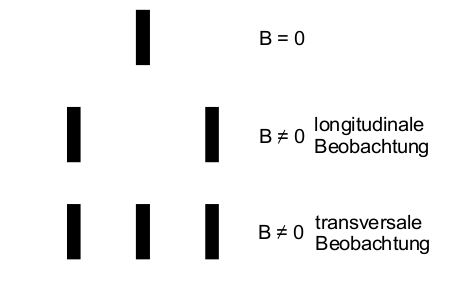
\includegraphics[width=0.7\columnwidth]{pictures/linien.png}
  \caption{Prinzipielles Aufspaltungsbild der Spektrallinien bei Anlegen eines Magnetfelds.\cite{Anleitung}}
  \label{fig:linien}
\end{figure}
Da die beiden Komponenten senkrecht zur Feldrichtung einen nicht verschwindenden Imaginärteil haben, ergibt sich für sie eine zirkular-polarisierte Schwingung um die Feldrichtung. Sie unterscheiden sich, abhängig vom $\Delta m=\pm 1$ in ihrer Drehrichtung und wird entsprechend als $^{+}\sigma$-, beziehungsweise als $^{-}\sigma$-Komponente bezeichnet.
Sie wirken in transversaler Beobachtung zum Magnetfeld ebenfalls linear polarisiert.
In ihrer Energie unterscheiden sie sich um jeweils $\mu_{\mathrm{B}}B$ von der unverschobenen Linie (siehe \ref{fig:linien}).

\subsection{Der normale Zeeman-Effekt}
Da die Schrödinger-Gleichung, welche Ausgangspunkt der bisherigen Überlegungen war, unabhängig vom Spin ist, sind die bisherigen Erkenntnisse auch nur für den Fall dass die Spinquantenzahl $S=0$ ist, gültig.
Dies wird als der normale Zeeman-Effekt bezeichnet. Der Landé-Faktor ist für diesen Fall nach Gleichung \eqref{eqn:lande} $g_{\mathrm{J}}=1$.
Die Aufspaltung der Energieniveaus erfolgt äquidistant nach Gleichung \eqref{eqn:Emag} mit $\Delta \mathrm{E}=m\cdot \mu_{\mathrm{B}}$.
Mit der Energie $E_0$ ohne Anwesenheit eines Magnetfelds ergibt sich die Energie der emittierten Spektrallinien zu:
\begin{equation}
  E=E_0+ m\cdot \mu_{\mathrm{B}}
\end{equation}
Aufgrund der äquidistanten Energieaufspaltung lassen sich also folglich für die verschiedenen Übergänge jeweils nur eine Spektrallinie beobachten (vgl. \ref{fig:normaler}).
\begin{figure}
  \centering
  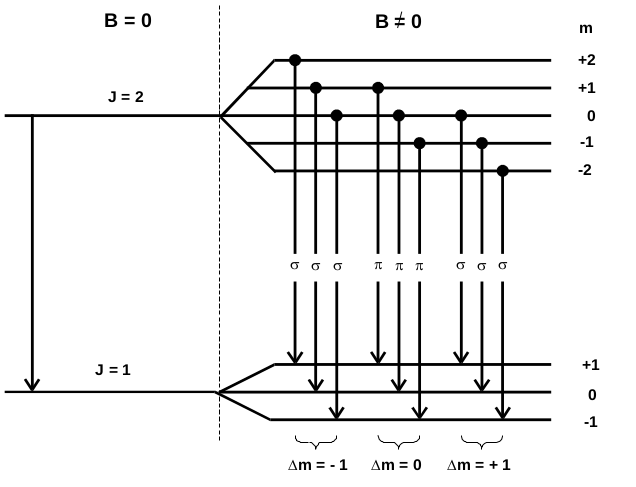
\includegraphics[width=0.75\columnwidth]{pictures/linienaufspaltung.png}
  \caption{Aufspaltung der Energieniveaus und mögliche Übergänge beim normalen Zeeman-Effekt.\cite{Anleitung}}
  \label{fig:normaler}
\end{figure}
\subsection{Der anomale Zeeman-Effekt}
In den bisherigen Überlegungen wurde der Spin zwar nicht berücksichtigt, es zeigt sich jedoch, dass auch wenn $S\neq 0$ ist, weiterhin die Auswahlregel $\Delta m=0 ; \pm 1$ gilt.
Da die Energieaufspaltung nun nicht mehr äquidistant ist, ist das Emissionsspektrum linienreicher.
Die Energie der emittierten Spektrallinie ist nun abhängig von den Landé-Faktoren $g_i$ der beteiligten Energieniveaus:
\begin{equation}
  \Delta E=\left(m_1g_1-m_2g_2\right)\mu_{\mathrm{B}}B+E_0
\end{equation}
Hierbei bezeichnen die $m_i$ die Orientierungsquantenzahlen der beteiligten Niveaus und $E_0$ die Energie bei ausgeschalteten B-Feld.

\subsection{Lummer-Gehrcke-Platte}
Zur Bestimmung der Wellenlängen der aufgespaltenen Spektrallinien, wird eine Lummer-Gehrcke-Platte verwendet.
Das emittierte Licht dringt in die Lummer-Gehrcke-Platte, welche aus zwei planparallelen Platten besteht ein und wird, wie in Abbildung \ref{fig:lummer} dargestellt, zwischen den Platten reflektiert.
\begin{figure}
  \centering
  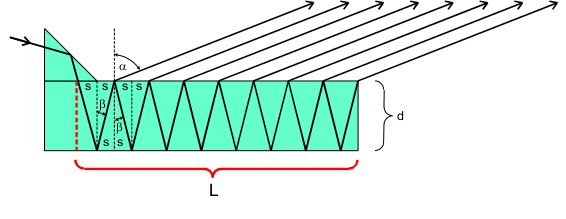
\includegraphics[width=0.7\columnwidth]{pictures/lummer.png}
  \caption{Strahlengang in der Lummer-Gehrcke-Platte zur Erzeugung der konstruktiven Interferenzen.\cite{Anleitung}}
  \label{fig:lummer}
\end{figure}
Bei der Reflektion an der Oberseite der Platte verlässt ein Teil des Lichts die Platte.
Die Lichtbündel, die hierbei entstehen, überlagern sich konstruktiv und bilden Interferenzstreifen. Der Abstand der Interferenzstreifen entspricht hierbei genau der eingestrahlten Wellenlänge $\lambda$.
Wird ein Magnetfeld angelegt, verschieben sich die Interferenzstreifen um $\Delta \lambda$.

Zwei Wellenlängen können nur aufgelöst werden, wenn der Wellenlängenunterschied mindestens
\begin{equation}
  \label{dispersionsgebiet}
	\Delta \lambda_{\mathrm{D}} = \frac{\lambda^2}{2d} \cdot \sqrt{\frac{1}{n^2 - 1}}
\end{equation}
beträgt.
Es ist $\Delta \lambda_{\mathrm{D}}$ das Dispersionsgebiet und $n$ der Brechungsindex, sowie $d$ die Dicke der Lummer-Gehrcke-Platte.
Das Auflösungsvermögen der Lummer-Gehrcke-Platte ist
\begin{equation}
  A=\frac{\lambda}{\Delta \lambda}=\frac{L}{\lambda}\left(n^2-1\right)\mathrm{.}
\end{equation}
Hierbei ist $L$ die Länge der Lummer-Gehrcke-Platte.
